\section{Date: 2026-11-11}
\noindent \textbf{Series ID: WUPIMMR} 

\noindent This series is titled World Pandemic Uncertainty Index for Myanmar and has a frequency of Quarterly. The units are Index and the seasonal adjustment is Not Seasonally Adjusted.The observation start date is 1996-01-01 and the observation end date is 2026-07-01.The popularity of this series is 1. \\ 

\noindent \textbf{Series ID: SFTPINDM114SFRBSF} 

\noindent This series is titled San Francisco Tech Pulse (DISCONTINUED) and has a frequency of Monthly. The units are Index Jan 2000=100 and the seasonal adjustment is Seasonally Adjusted.The observation start date is 1971-04-01 and the observation end date is 2020-03-01.The popularity of this series is 9. \\ 

\subsection{Raw Regression}
\noindent Regresses the two series against each other directly. A significant result here can come just as easily from both series sharing a long-run trend as from any real relationship.

\begin{center}
\begin{tabular}{lclc}
\toprule
\textbf{Dep. Variable:}       & value\_fred\_SFTPINDM114SFRBSF & \textbf{  R-squared:         } &     0.024   \\
\textbf{Model:}               &              OLS               & \textbf{  Adj. R-squared:    } &     0.013   \\
\textbf{Method:}              &         Least Squares          & \textbf{  F-statistic:       } &     2.309   \\
\textbf{Date:}                &        Wed, 11 Nov 2026        & \textbf{  Prob (F-statistic):} &    0.132    \\
\textbf{Time:}                &            18:56:01            & \textbf{  Log-Likelihood:    } &   -381.14   \\
\textbf{No. Observations:}    &                 97             & \textbf{  AIC:               } &     766.3   \\
\textbf{Df Residuals:}        &                 95             & \textbf{  BIC:               } &     771.4   \\
\textbf{Df Model:}            &                  1             & \textbf{                     } &             \\
\textbf{Covariance Type:}     &           nonrobust            & \textbf{                     } &             \\
\bottomrule
\end{tabular}
\begin{tabular}{lcccccc}
                              & \textbf{coef} & \textbf{std err} & \textbf{t} & \textbf{P$> |$t$|$} & \textbf{[0.025} & \textbf{0.975]}  \\
\midrule
\textbf{const}                &      83.0755  &        1.269     &    65.444  &         0.000        &       80.555    &       85.596     \\
\textbf{value\_fred\_WUPIMMR} &      -0.2581  &        0.170     &    -1.519  &         0.132        &       -0.595    &        0.079     \\
\bottomrule
\end{tabular}
\begin{tabular}{lclc}
\textbf{Omnibus:}       &  4.185 & \textbf{  Durbin-Watson:     } &    0.129  \\
\textbf{Prob(Omnibus):} &  0.123 & \textbf{  Jarque-Bera (JB):  } &    3.548  \\
\textbf{Skew:}          &  0.445 & \textbf{  Prob(JB):          } &    0.170  \\
\textbf{Kurtosis:}      &  3.296 & \textbf{  Cond. No.          } &     7.51  \\
\bottomrule
\end{tabular}
%\caption{OLS Regression Results}
\end{center}

Notes: \newline
 [1] Standard Errors assume that the covariance matrix of the errors is correctly specified.

\begin{figure}
\centering
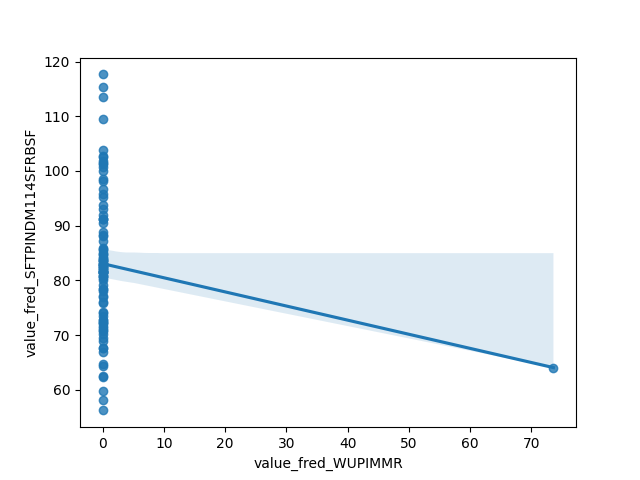
\includegraphics[scale = 0.9]{plots/plot_2026-11-11.png}
\caption{Raw Regression Plot for 2026-11-11}
\end{figure}
\newpage
\subsection{Detrended Regression}
\noindent Regresses the residuals of each series after removing its own linear time trend, so a shared trend can no longer drive the result on its own. A relationship that stays significant here is better evidence of a genuine link between the two series.

\begin{center}
\begin{tabular}{lclc}
\toprule
\textbf{Dep. Variable:}                  & value\_fred\_SFTPINDM114SFRBSF\_detrended & \textbf{  R-squared:         } &     0.019   \\
\textbf{Model:}                          &                    OLS                    & \textbf{  Adj. R-squared:    } &     0.009   \\
\textbf{Method:}                         &               Least Squares               & \textbf{  F-statistic:       } &     1.861   \\
\textbf{Date:}                           &              Wed, 11 Nov 2026             & \textbf{  Prob (F-statistic):} &    0.176    \\
\textbf{Time:}                           &                  18:56:01                 & \textbf{  Log-Likelihood:    } &   -374.38   \\
\textbf{No. Observations:}               &                       97                  & \textbf{  AIC:               } &     752.8   \\
\textbf{Df Residuals:}                   &                       95                  & \textbf{  BIC:               } &     757.9   \\
\textbf{Df Model:}                       &                        1                  & \textbf{                     } &             \\
\textbf{Covariance Type:}                &                 nonrobust                 & \textbf{                     } &             \\
\bottomrule
\end{tabular}
\begin{tabular}{lcccccc}
                                         & \textbf{coef} & \textbf{std err} & \textbf{t} & \textbf{P$> |$t$|$} & \textbf{[0.025} & \textbf{0.975]}  \\
\midrule
\textbf{const}                           &     7.54e-13  &        1.178     &   6.4e-13  &         1.000        &       -2.338    &        2.338     \\
\textbf{value\_fred\_WUPIMMR\_detrended} &      -0.2166  &        0.159     &    -1.364  &         0.176        &       -0.532    &        0.099     \\
\bottomrule
\end{tabular}
\begin{tabular}{lclc}
\textbf{Omnibus:}       & 26.198 & \textbf{  Durbin-Watson:     } &    0.131  \\
\textbf{Prob(Omnibus):} &  0.000 & \textbf{  Jarque-Bera (JB):  } &   39.153  \\
\textbf{Skew:}          &  1.224 & \textbf{  Prob(JB):          } & 3.15e-09  \\
\textbf{Kurtosis:}      &  4.922 & \textbf{  Cond. No.          } &     7.42  \\
\bottomrule
\end{tabular}
%\caption{OLS Regression Results}
\end{center}

Notes: \newline
 [1] Standard Errors assume that the covariance matrix of the errors is correctly specified.

\begin{figure}
\centering
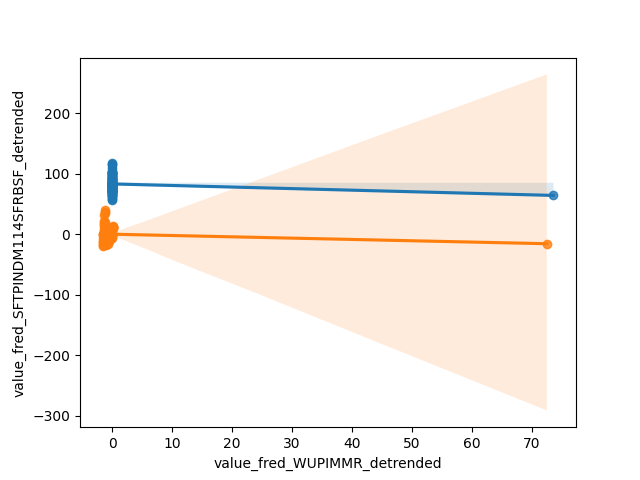
\includegraphics[scale = 0.9]{plots/plot_2026-11-11_detrended.png}
\caption{Detrended Regression Plot for 2026-11-11}
\end{figure}
\newpage
